\documentclass[10pt,a4paper]{article}
\usepackage[margin=2.2cm]{geometry}
\usepackage{fontspec}
\usepackage{kotex}
\setmainfont{Apple SD Gothic Neo}
\setsansfont{Apple SD Gothic Neo}
\usepackage{amsmath,amssymb}
\usepackage{graphicx}
\usepackage{booktabs}
\usepackage{caption}
\usepackage[dvipsnames]{xcolor}
\usepackage[colorlinks=true,linkcolor=MidnightBlue,citecolor=MidnightBlue,
            urlcolor=MidnightBlue]{hyperref}
\usepackage{titlesec}
\titleformat{\section}{\large\bfseries}{\thesection}{0.6em}{}
\titleformat{\subsection}{\normalsize\bfseries}{\thesubsection}{0.5em}{}
\captionsetup{font=small,labelfont=bf}
\setlength{\parskip}{0.35em}
\setlength{\parindent}{0pt}

\usepackage{mdframed}
\newmdenv[linewidth=0.4pt,linecolor=gray!60,backgroundcolor=gray!5,
          innertopmargin=6pt,innerbottommargin=6pt,skipabove=8pt,skipbelow=8pt]{claimbox}
\newcommand{\claim}[2]{\begin{claimbox}\textbf{주장.} #1\par\smallskip
  \textcolor{gray!70}{\textbf{반증 조건.} #2}\end{claimbox}}

\title{\bfseries 여덟은 거꾸로 간다\\[2pt]
\large 도메인을 하나씩 빼 보니 순수 전이가 되는 것은 일본 만화·애니 계열 셋뿐이었다}
\author{월드모델 실험실 · 노트 722 · 723}
\date{2026-08-06}
\begin{document}\maketitle

\section{한 줄}

공유 트렁크에서 \textbf{도메인을 하나씩 빼고} 다시 적합해 그 도메인 예보를 쟀다
(LODO). \textbf{자기 행이 하나도 안 든 트렁크가 양의 예보를 주는 도메인은 셋뿐}이고
\textbf{여덟은 음수} --- 전이가 안 되는 게 아니라 \textbf{거꾸로 간다}. 그리고 그
셋은 다 \textbf{일본 만화·애니 계열}이다.

\section{왜 하나씩 뺐나}

노트 721 이 \textbf{시장팝업 하나가 공유 표현의 이득을 독점}하는 것을 쟀다
(신호 몫 $+0.1857$ · 자기 문턱의 $7.98$배 · 판 기여 $66\%$). 노트 698 에서도
같았다($+0.1534$). T5 의 다음 실험이 \emph{``시장팝업을 빼고 다시 적합''} 이었는데
\textbf{전 도메인으로 일반화했다} --- 도메인 하나로 결론 내지 말라는 노트 646 을
지키면서 $n{=}1$ 대신 $n{=}11$ 을 얻는다.

읽는 자를 셋으로 갈랐다.

\begin{center}
\begin{tabular}{ll}
\toprule
\textbf{전부} & 그 도메인이 지금 받는 예보 품질 \\
\textbf{LODO} & \textbf{자기 행이 하나도 안 든} 트렁크의 품질 $\to$ \textbf{순수 전이} \\
$\Delta$ & 전부 $-$ LODO $=$ 자기 행이 보탠 몫 \\
\bottomrule
\end{tabular}
\end{center}

판 적합은 안 했다 --- 축 품질을 직접 재므로 트렁크(2{,}497 모수)만 12회 $\times$
씨앗 4 돌리면 끝난다. \textbf{어휘와 SVD 는 전부 넣은 학습 행으로 한 번만 만들었다}
--- 그것까지 빼면 ``표현이 없어서''와 ``신경망이 못 배워서''가 섞인다.

\begin{figure}[t]\centering
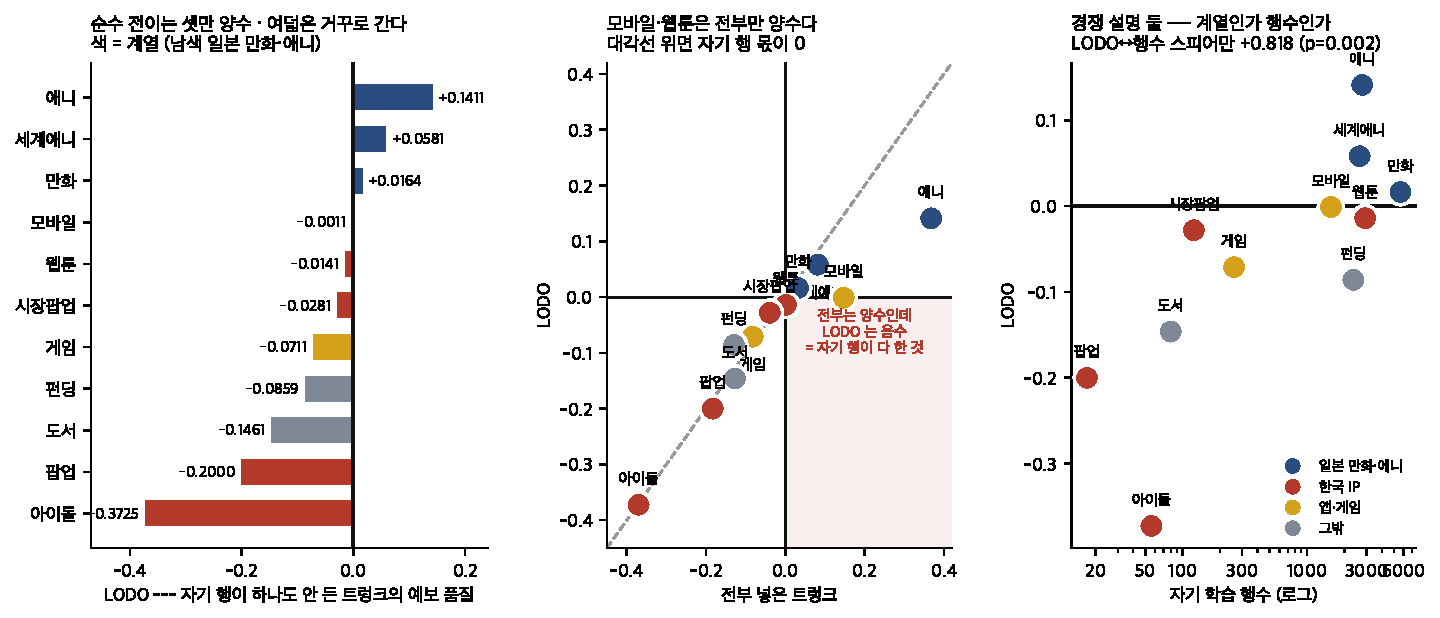
\includegraphics[width=0.99\textwidth]{figs/backwards.pdf}
\caption{왼쪽: LODO --- \textbf{셋만 양수}이고 색이 계열이다. 가운데: 전부 대 LODO
--- \textbf{모바일·웹툰은 전부만 양수}다(자기 행이 다 했다). 오른쪽: 경쟁 설명 둘
--- 계열인가 행수인가.}
\end{figure}

\section{순수 전이가 되는 것은 셋뿐이다}

\begin{center}
\begin{tabular}{lrrrrl}
\toprule
도메인 & 전부 & \textbf{LODO} & $\Delta$ & 학습 & 계열 \\
\midrule
애니 & $+0.3680$ & $\mathbf{+0.1411}$ & $+0.2269$ & $2{,}779$ & 일본 만화·애니 \\
세계애니 & $+0.0821$ & $\mathbf{+0.0581}$ & $+0.0240$ & $2{,}647$ & 일본 만화·애니 \\
만화 & $+0.0322$ & $\mathbf{+0.0164}$ & $+0.0158$ & $5{,}644$ & 일본 만화·애니 \\
\midrule
모바일 & $+0.1473$ & $-0.0011$ & $+0.1484$ & $1{,}558$ & 앱·게임 \\
웹툰 & $+0.0015$ & $-0.0141$ & $+0.0156$ & $2{,}936$ & 한국 IP \\
시장팝업 & $-0.0393$ & $-0.0281$ & $-0.0112$ & $123$ & 한국 IP \\
게임 & $-0.0824$ & $-0.0711$ & $-0.0113$ & $259$ & 앱·게임 \\
펀딩 & $-0.1292$ & $-0.0859$ & $-0.0433$ & $2{,}358$ & 그밖 \\
도서 & $-0.1270$ & $-0.1461$ & $+0.0192$ & $80$ & 그밖 \\
팝업 & $-0.1832$ & $-0.2000$ & $+0.0168$ & $17$ & 한국 IP \\
아이돌 & $-0.3704$ & $-0.3725$ & $+0.0021$ & $56$ & 한국 IP \\
\bottomrule
\end{tabular}
\end{center}

\claim{\textbf{공유 표현은 하나의 IP 계열 안에서만 옮겨간다.} LODO 양수 셋이 다
일본 만화·애니 계열이고, \textbf{웹툰은 $2{,}936$행인데도 $-0.0141$} 이다 ---
행수가 아니라 계열이 정한다. 그러므로 ``하나의 파운데이션''은 지금 자료에서
\textbf{계열 단위로만} 성립한다.}
{\textbf{경쟁 설명이 있고 이 자료로는 못 가른다} --- LODO $\leftrightarrow$ 학습
행수 스피어만이 $+0.818$($p{=}0.002$)다. 큰 도메인이 곧 만화·애니 계열이라
\textbf{계열과 크기가 교란돼 있다.} 계열 안에서만 공유하는 트렁크를 계열마다
적합해 LODO 가 오르면 계열 가설이 서고, 안 오르면 크기가 답이다.}

\subsection*{음수는 ``전이 안 됨''이 아니라 ``거꾸로 감''이다}

여덟 도메인에서 \textbf{다른 도메인만으로 학습한 트렁크가 라벨과 음의 상관}을
낸다(팝업 $-0.2000$ · 아이돌 $-0.3725$ · 도서 $-0.1461$). \textbf{0 이 아니라
음수라는 것이 핵심이다.}

\claim{\textbf{이것은 입문서 04면이 잰 기제와 같다} --- \emph{``방향이 없으면
전이도 없다''}. 도메인마다 텍스트$\to$라벨 방향이 다르면 합친 트렁크가 어떤
도메인에서는 반대로 간다. \textbf{그때 처방은 가리는 것이 아니라 방향을 세우는
것}이었고(노트 604 계열), 여기서도 같은 처방이 필요하다.}
{음수가 씨앗 잡음일 수 있다. 아이돌은 유보 51행이라 자기 문턱이 크다 ---
$0.0045\sqrt{3369/51} = 0.0366$ 이고 $-0.3725$ 는 그 열 배 밖이므로 잡음이 아니다.
반면 웹툰 $-0.0141$ 은 자기 문턱 $0.0102$ 의 $1.4$배로 얇다.}

\section{노트 721 의 해석을 정정한다}

노트 721 은 시장팝업 신호 몫 $+0.1857$ 을 \emph{``공유 표현의 이득을 독점한다''}고
읽었다. \textbf{그런데 그 도메인의 축 품질 자체가 $-0.0393$ 으로 음수다.}

\claim{\textbf{판은 트리 모형이라 음의 상관을 뒤집어 쓸 수 있다.} 그러므로 그 이득은
``좋은 예보''가 아니라 \textbf{``판이 쓸 수 있는 어떤 신호''}다.
\textbf{``독점한다''는 맞고 ``이득을 본다''는 틀렸다.} 모바일도 같은 자리다 ---
전부 $+0.1473$ 인데 LODO $-0.0011$ 이라 \textbf{자기 행이 전부 다 했다.}}
{축 품질을 도메인 안 스피어만으로 쟀다. 판이 실제로 쓰는 것은 다른 열들과의
상호작용이라, 단독 상관이 음수여도 조건부로는 양수일 수 있다 --- 그 경우 ``뒤집어
쓴다''가 아니라 ``다른 열과 함께 쓴다''가 맞는 서술이 된다.}

\subsection*{그래서 조항이 하나 생겼다}

\begin{center}
\textbf{신호 몫을 보고할 때 그 도메인의 축 품질을 같이 적는다.}\\
부호가 갈리면 ``판이 쓸 수 있다''까지만 말한다.
\end{center}

\section{예측 채점 --- 둘 틀리고 하나 맞았다}

\begin{center}
\begin{tabular}{lll}
\toprule
예측 & 결과 & \\
\midrule
$\Delta$ 가 자기 학습 행수와 함께 커진다 & 스피어만 $+0.173$ ($p{=}0.61$) & \textbf{틀림} \\
시장팝업 LODO 가 전부의 $70\%$ 이상 유지 & 유지율 $0.715$ & \textbf{수치만 맞음} \\
웹툰 $\Delta$ $>$ 시장팝업 $\Delta$ & $+0.0156$ 대 $-0.0112$ & \textbf{맞음} \\
\bottomrule
\end{tabular}
\end{center}

두 번째가 내 잘못이다. \textbf{유지율 $0.715$ 는 분자와 분모가 \emph{둘 다 음수}여서
양수로 나온 것}이다($-0.0281 / -0.0393$). 사전등록의 ``$70\%$ 이상 유지'' 조건이
\textbf{뜻 없이 충족됐다.}

\claim{\textbf{비율을 자로 세울 때 분모의 부호와 $0$ 근접을 먼저 검사한다.} 부호를
안 보면 ``많이 유지됐다''와 ``둘 다 거꾸로 간다''를 구분할 수 없다. 이것은 노트
715 · 717 이 문턱을 눈금한 것과 같은 층의 일이다 --- \textbf{자를 세울 때 그 자가
언제 무의미해지나를 같이 적어야 한다.}}
{비율 대신 차($\Delta$)만 쓰면 이 문제가 없다. 다만 차는 크기 비교가 안 되므로
정규화가 필요하고, 그 정규화가 다시 분모 문제를 부른다 --- 그래서 ``검사한다''가
``쓰지 않는다''보다 낫다.}

\end{document}
